
To properly evaluate practical downstream metrics described in section \ref{section:model-evaluation} on model predictions, one need to be able to segment nuclei from fluorescence (as well as from predictions) first. By segmentation here the creation of mask is understood. It should constist of $0$s and $1$s, with $1$ assigned to pixels that are part of nucleus and $0$ otherwise. Altough this might be a straight-forward task for our eyes, it is not that easy to select separate nuclei via post-processing. There are several edge cases where the nuclei are difficult to segment.

Even though the most extreme corruptions mentioned in section \ref{section:nuclei-preprocessing} were filtered out, some of the images that are corrupted not that severely (meaning they still have all the visible features needed for learning) are still present in the dataset. This allows to not reduce the amount of data  significantly.
\begin{figure}[H]
    \centering
    \setkeys{Gin}{width=\linewidth}
    \centering
        \begin{tabularx}{\textwidth}{YYYY}
            \textbf{Too few cells} &
            \textbf{Overexposure} &
            \textbf{Light gradient} &
            \textbf{Normal lightning} \\
            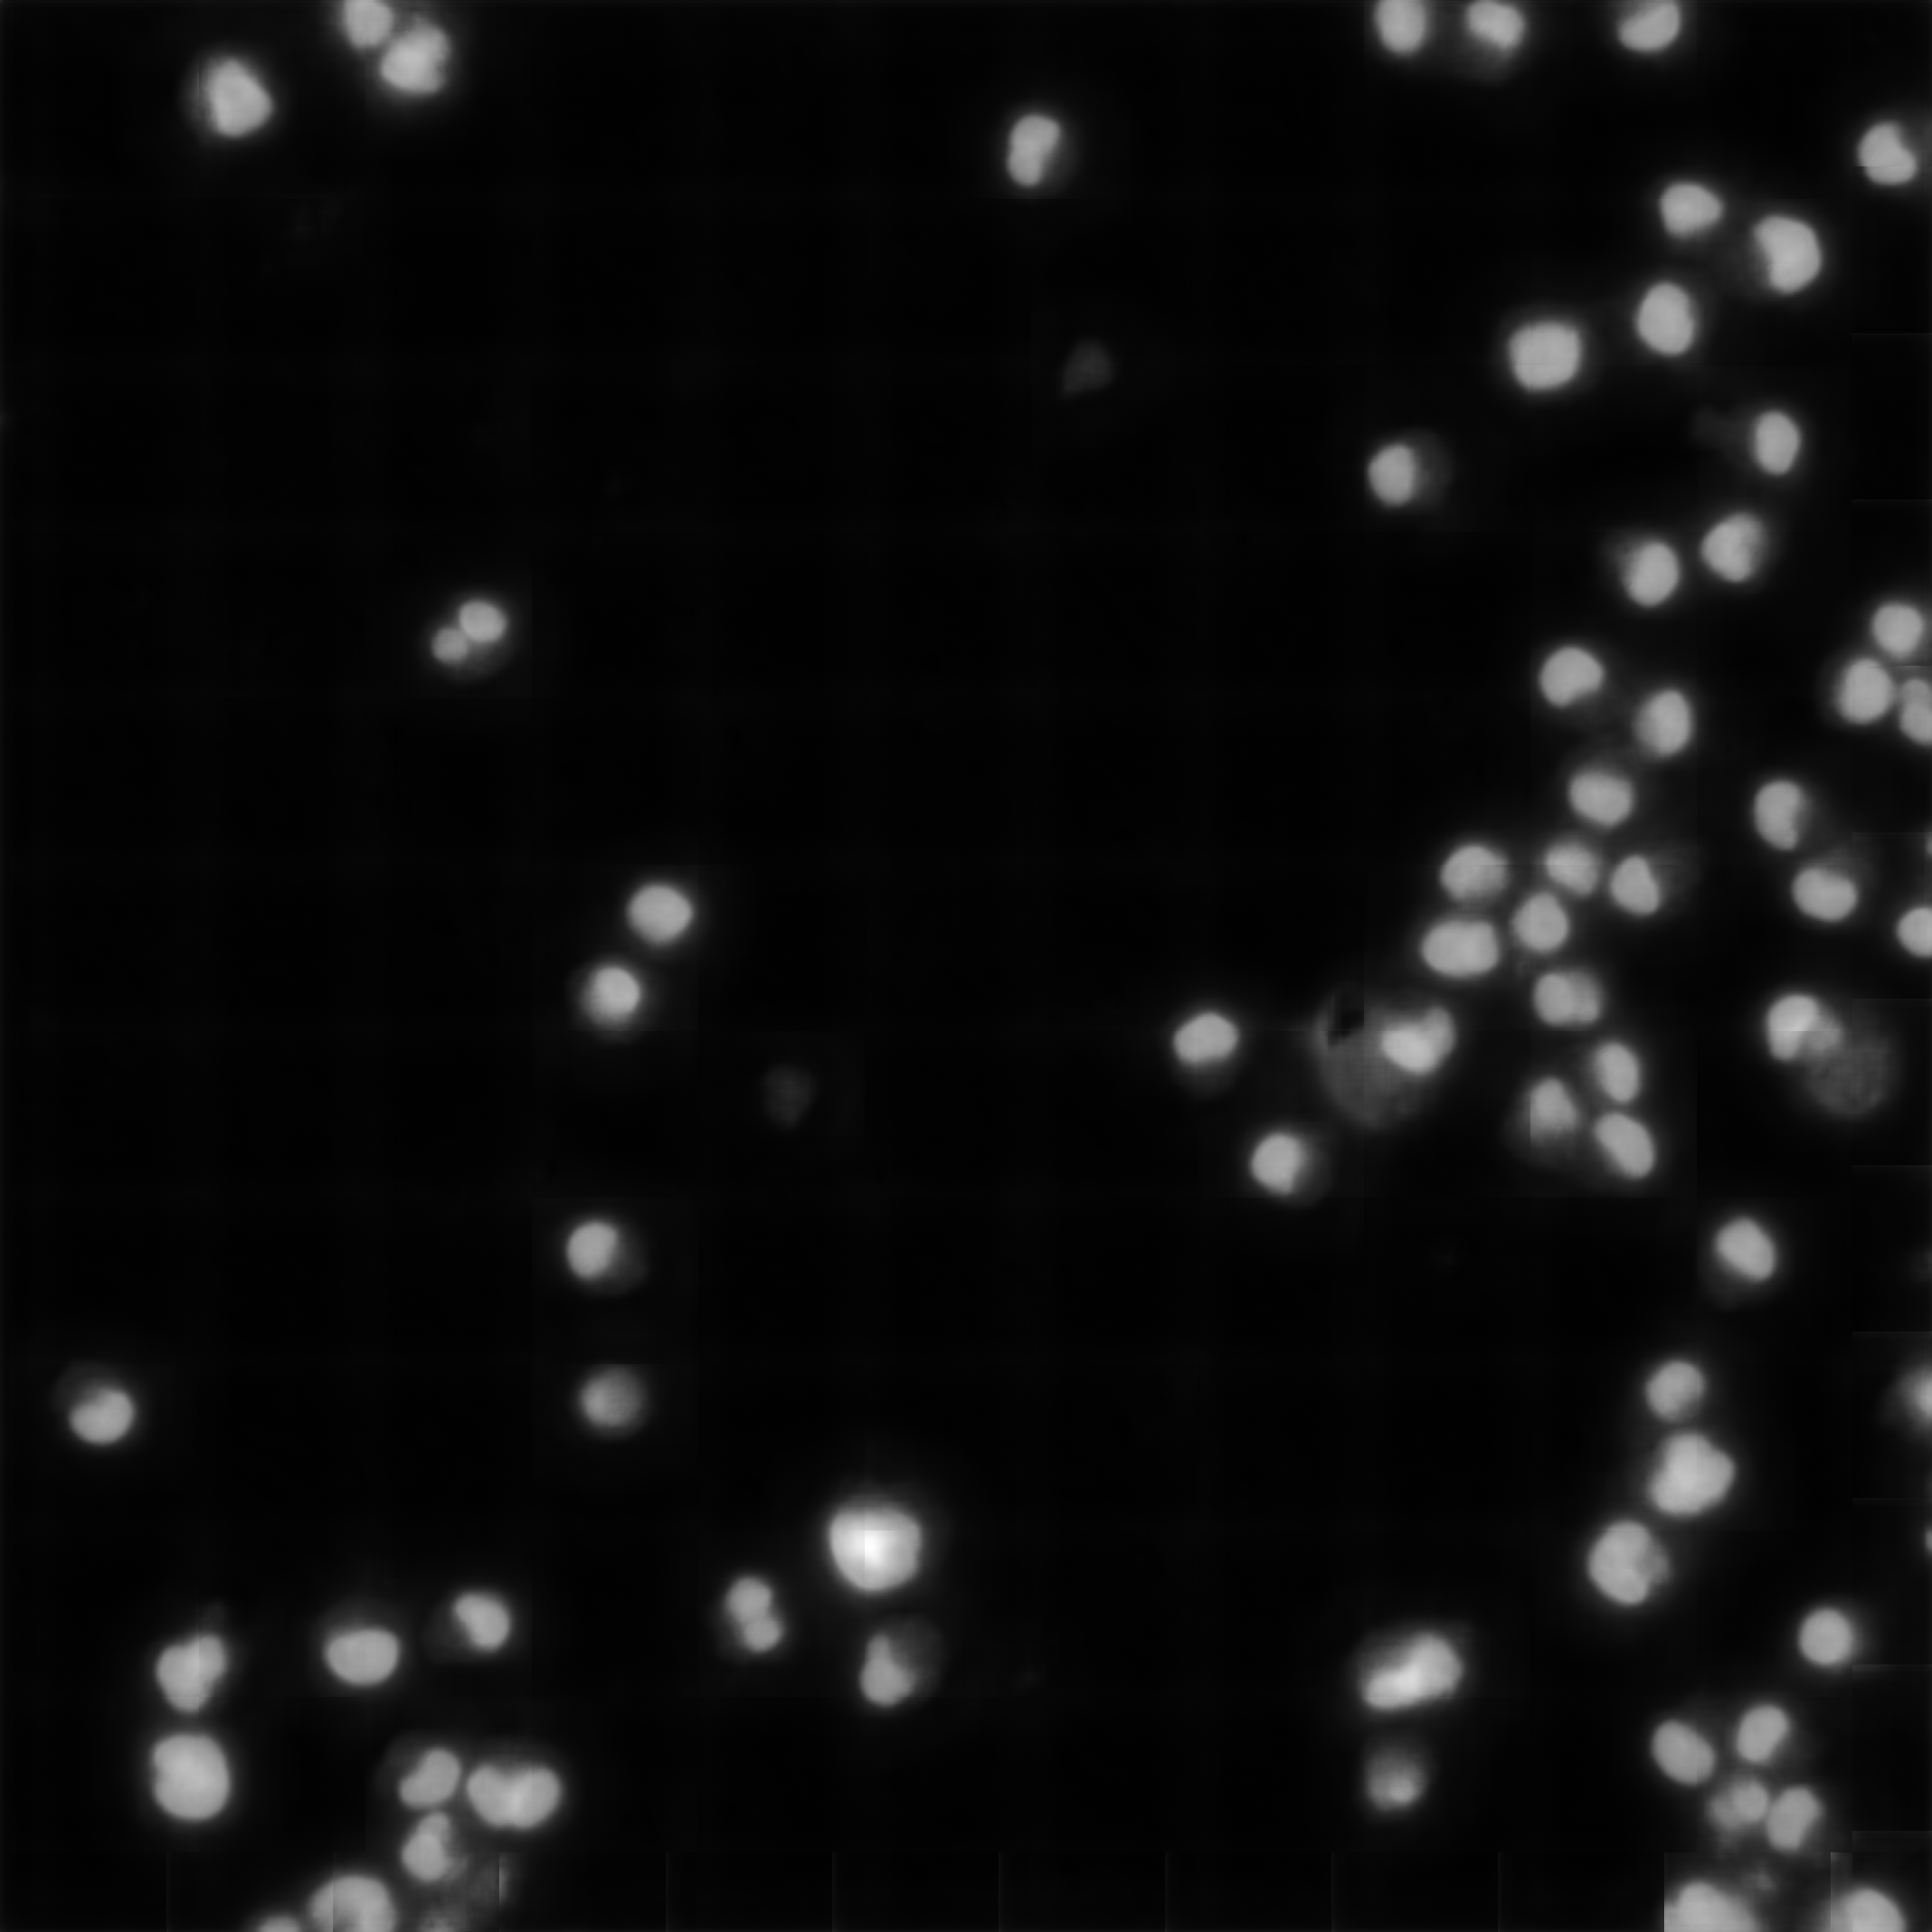
\includegraphics{bilder/lightning-conditions/lightning-1.png} & 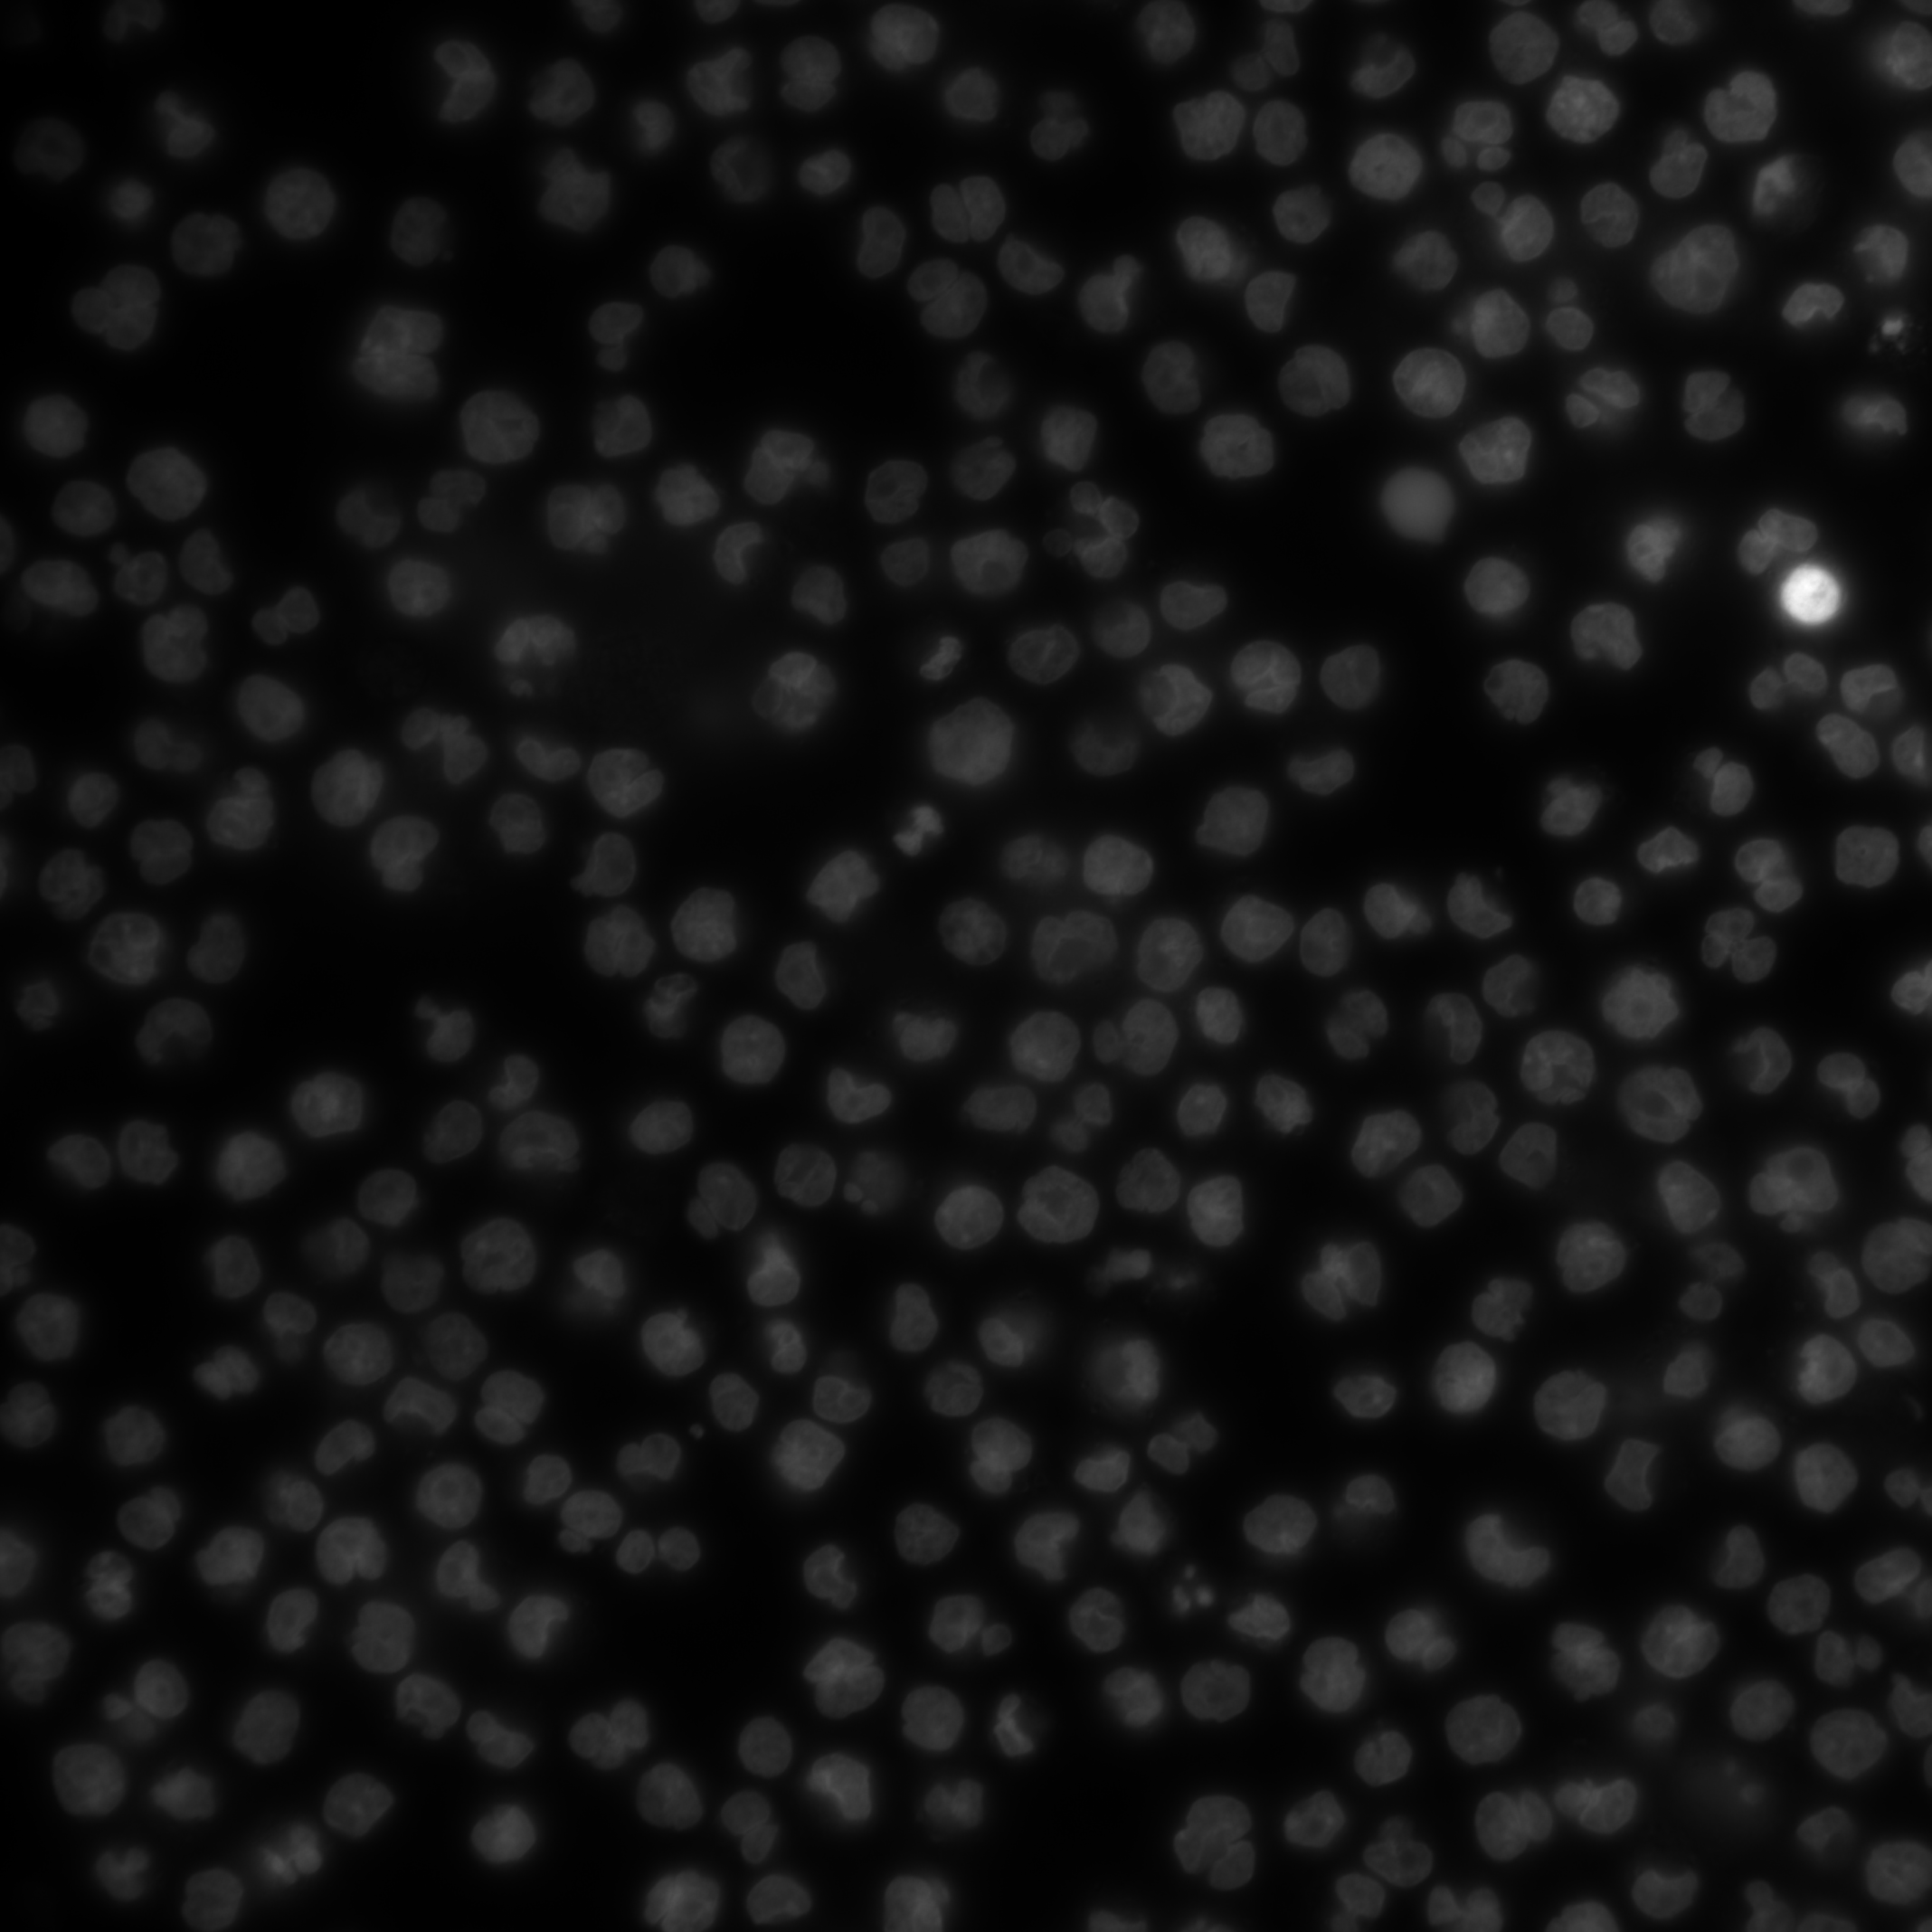
\includegraphics{bilder/lightning-conditions/lightning-2.png} &
            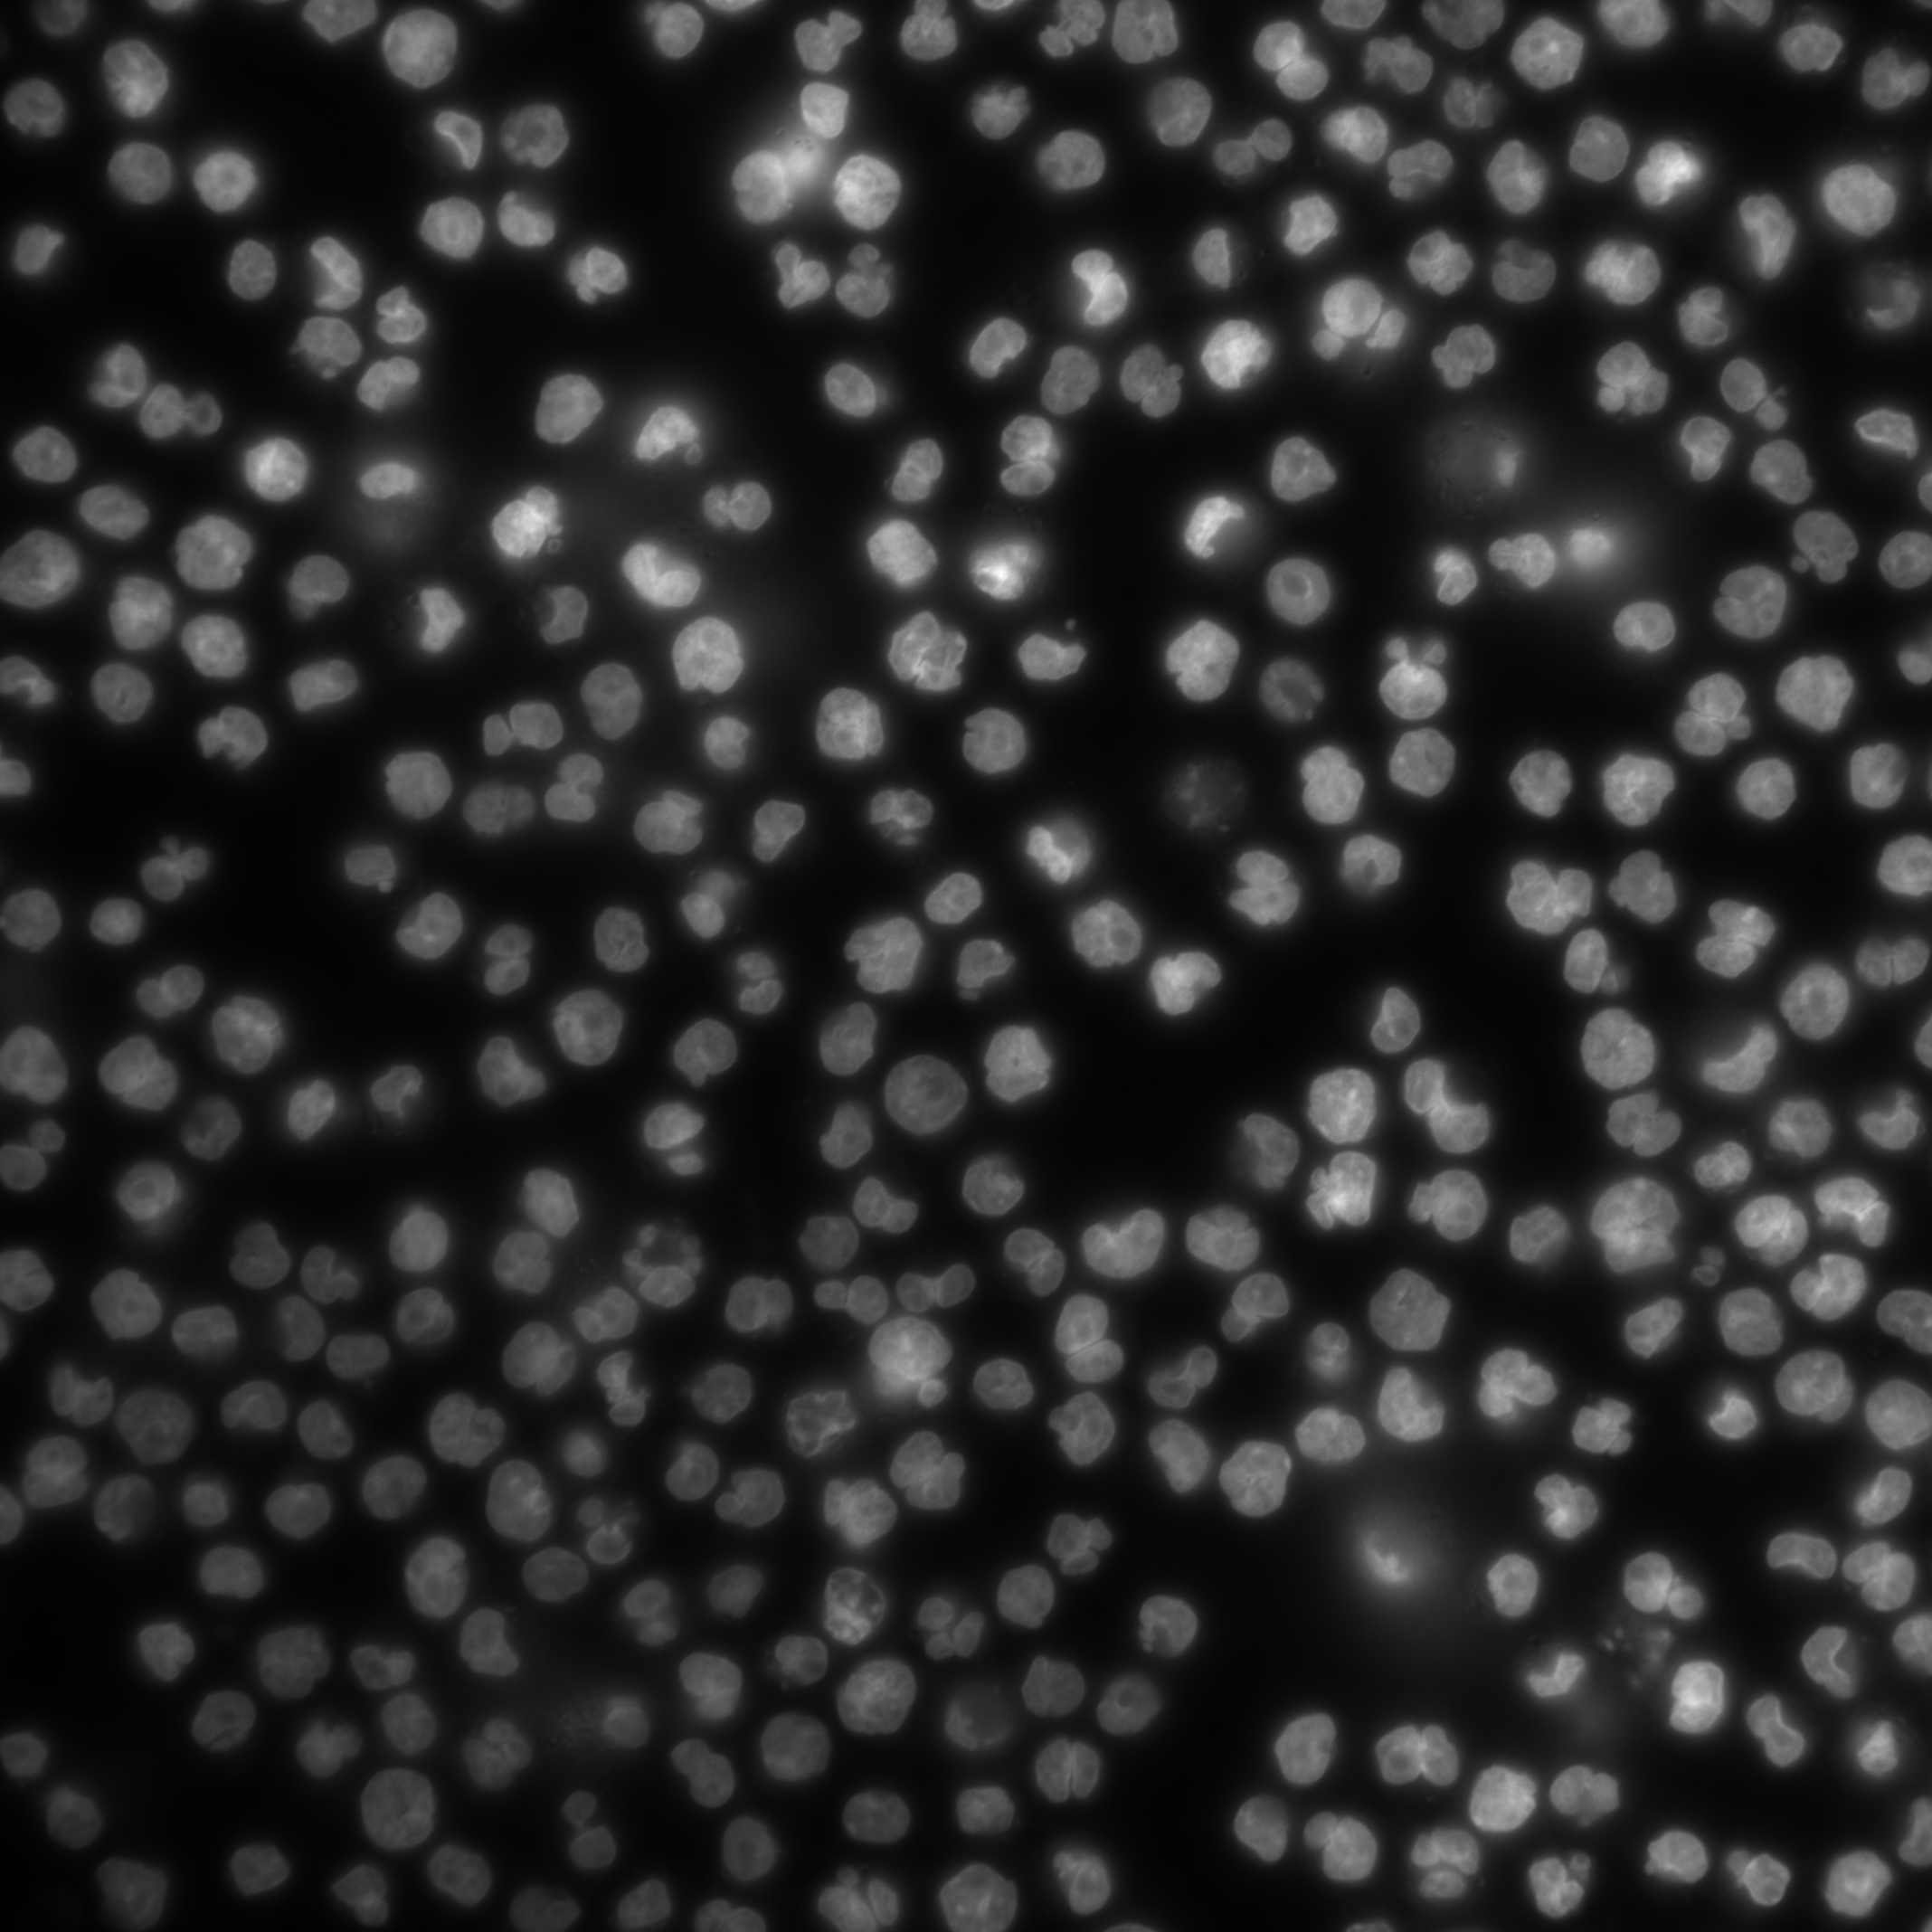
\includegraphics{bilder/lightning-conditions/lightning-3.png} & 
            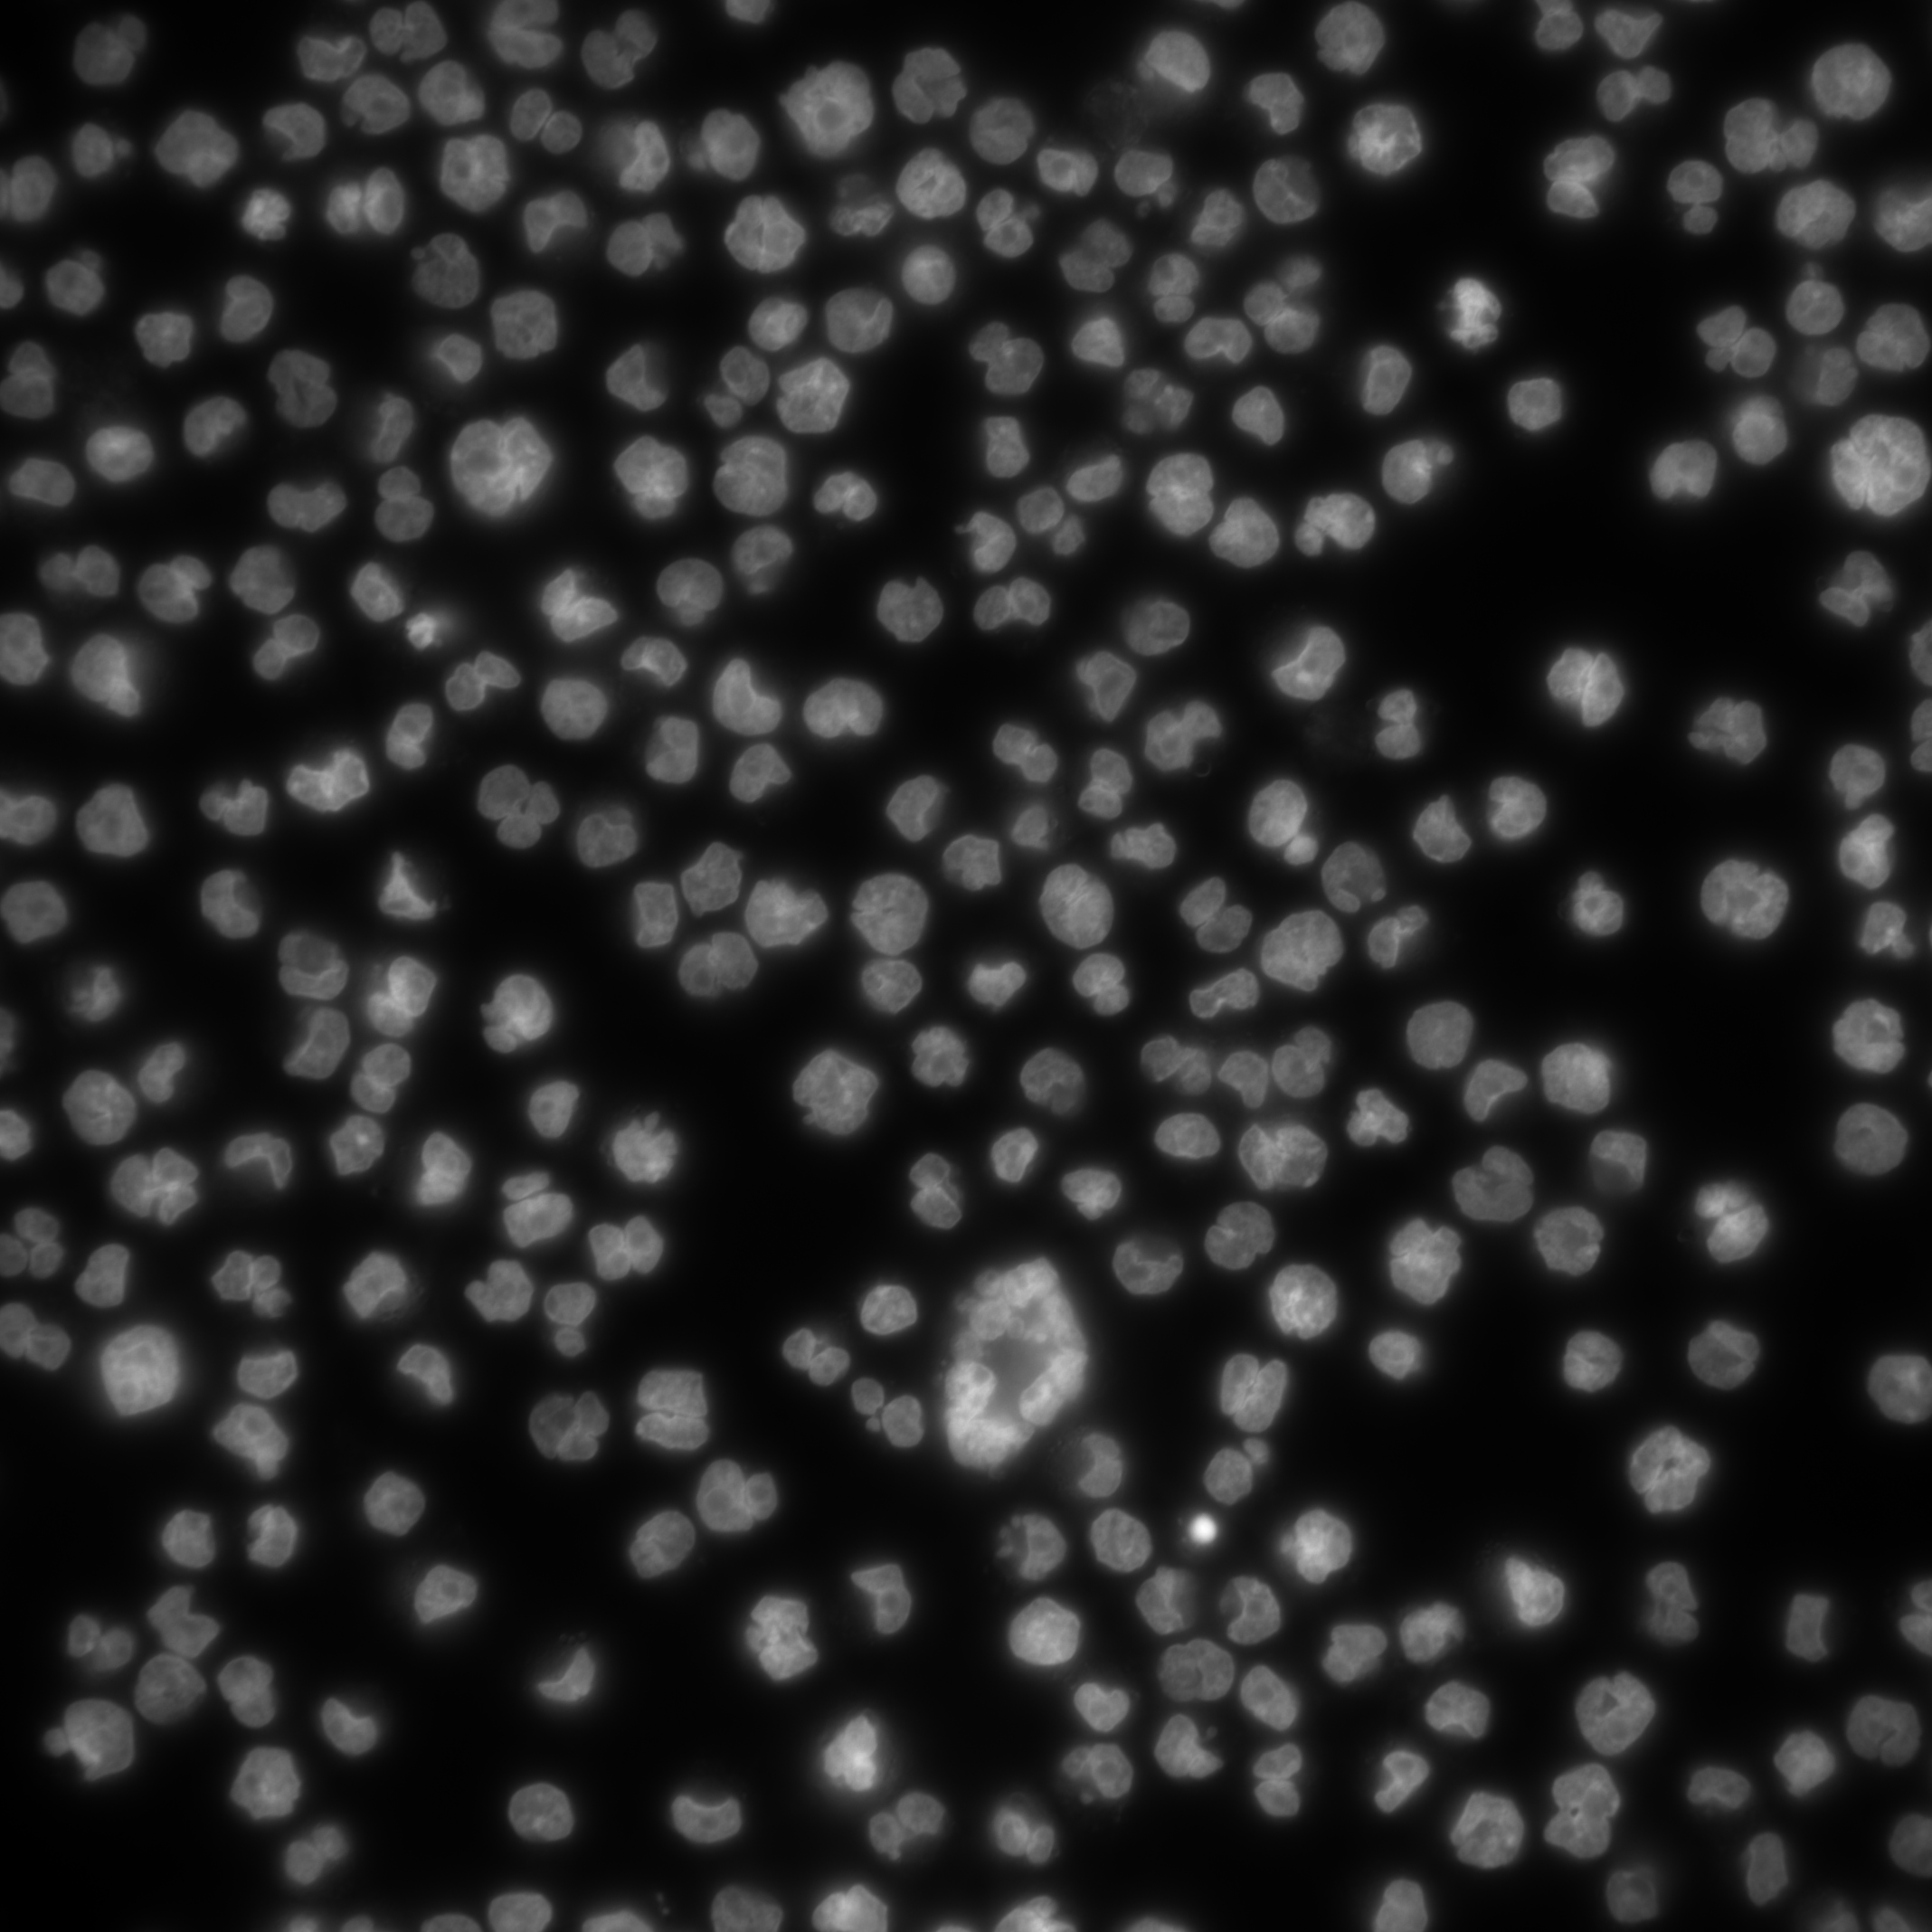
\includegraphics{bilder/lightning-conditions/lightning-4.png}
        \end{tabularx}
    \caption{Different lightning conditions}
    \label{fig:lightning_conditions}
\end{figure}

The examples of difficult for segmentation cases are presented in Figure \ref{fig:lightning_conditions} from left to right: image contains too few cells, which leads to background being much darker than usually; overexposure of one cell, which leads to difficulties of segmenting the rest of the cells as they are hard distinguishable from the background; lighting gradient from darker (left bottom corner) to brighter (upper right corner) region; normal lighting conditions.

Another challenge for segmentation bring nuclei that are very close to each other. This might happen sometimes because some of the cells are currently in the process of the division. Also when some have already fully divided, they might still be located close to one another. The example of such situations is presented in Figure \ref{fig:closely-located-cells}.

\begin{figure}[H]
    \centering
    \subfloat[Original fluorescence]{{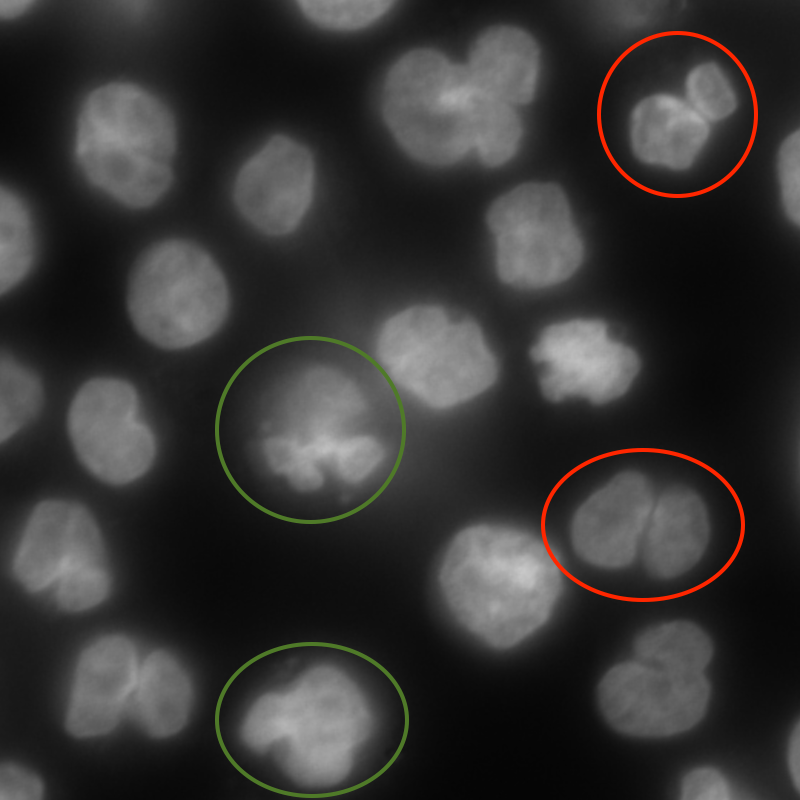
\includegraphics[width=0.2\linewidth]{bilder/close-located-cells/original.png} }}
    \qquad
    \subfloat[Segmentation (violet mask)]{{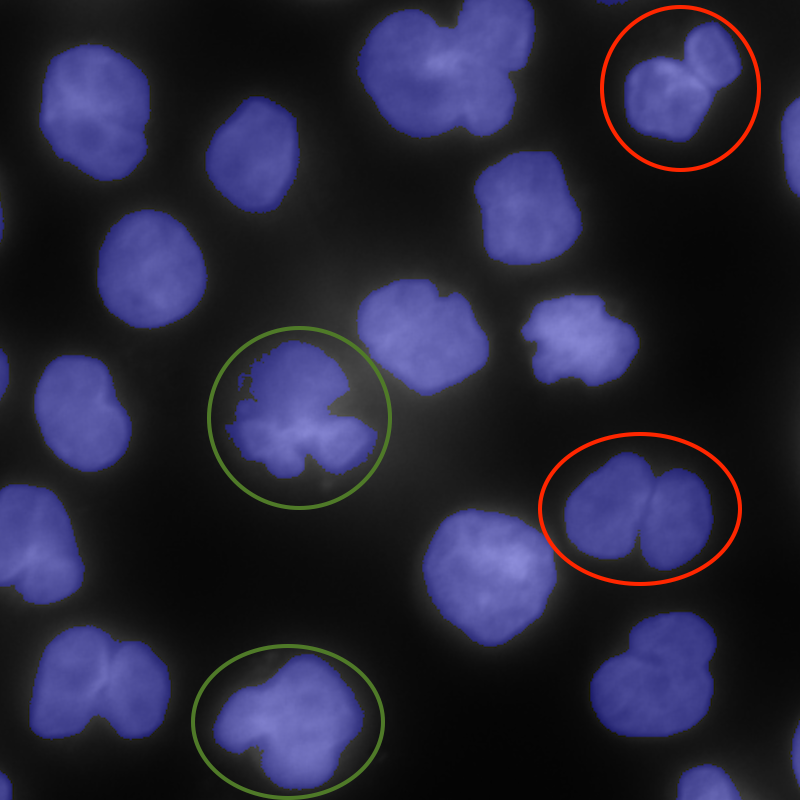
\includegraphics[width=0.2\linewidth]{bilder/close-located-cells/segmented.png} }}
    \caption{Closely located and dividing cells}
    \label{fig:closely-located-cells}
\end{figure}

Here cells, that are not yet fully divided are highlighted with the green cirles, and ones, that are fully divided, but just located too close to one another are highlighted with red circles. You can see that the segmentation algorithm (see Algorithm \ref{algorithm:nuclei-segmentation}) recognises both such cases as one nuclei. This algorithm is described below and its step are vidualized in Figure \ref{fig:segmentation-nuclei-steps}.
\begin{algorithm}
    \caption{Fluorescence segmentation}
    \begin{algorithmic}
    \item 1. Normalize image.
    \item 2. Apply local thresholding and get a threshold $T$ or a set of local thresholds \{$T_i$\} and create an initial mask: $1$ if $x_i > T$ or $0$ otherwise.  
    \item 3. Apply \textit{fill\_holes} transformation to the initial mask in order to get rid of unneeded details insides the nuclei.
    \item 4. Run \textit{findContours} from opencv in order to obtain separate regions and filter them based on the following criteria: filter out too big regions (measure the biggest possible nuclei manually), too small regions (measured manually as well), regions that have a shape that it not very similar to convex circular type of nuclei. The last filter is done by checking the ratio of the area of the region to the area of the convex hull of the region. 
    \end{algorithmic}
    \label{algorithm:nuclei-segmentation}
\end{algorithm}    

\begin{figure}[htb]
    \centering
    \setkeys{Gin}{width=\linewidth}
    \centering
        \begin{tabularx}{\textwidth}{YYYY}
            \textbf{Normalized input} &
            \textbf{Local threshold} &
            \textbf{Filled holes} &
            \textbf{Filtered regions} \\
            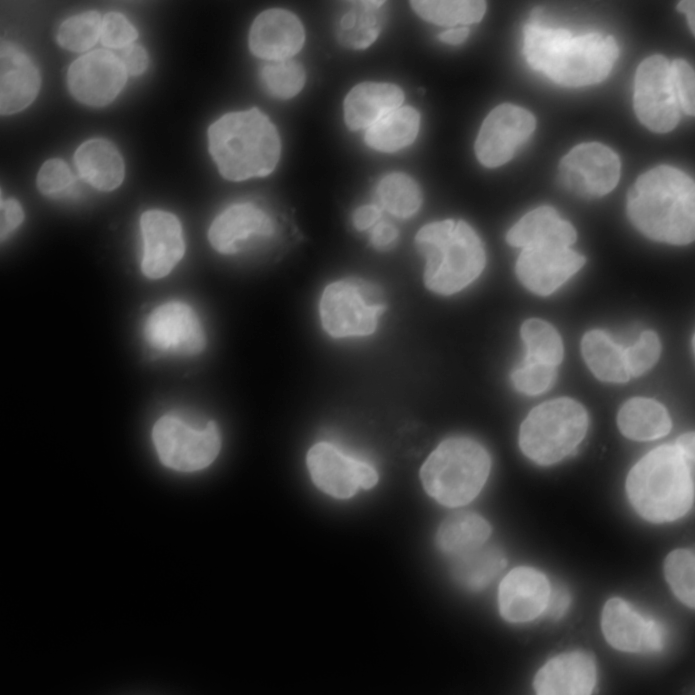
\includegraphics{bilder/segmentation/nuclei-mask/normalized.png} & 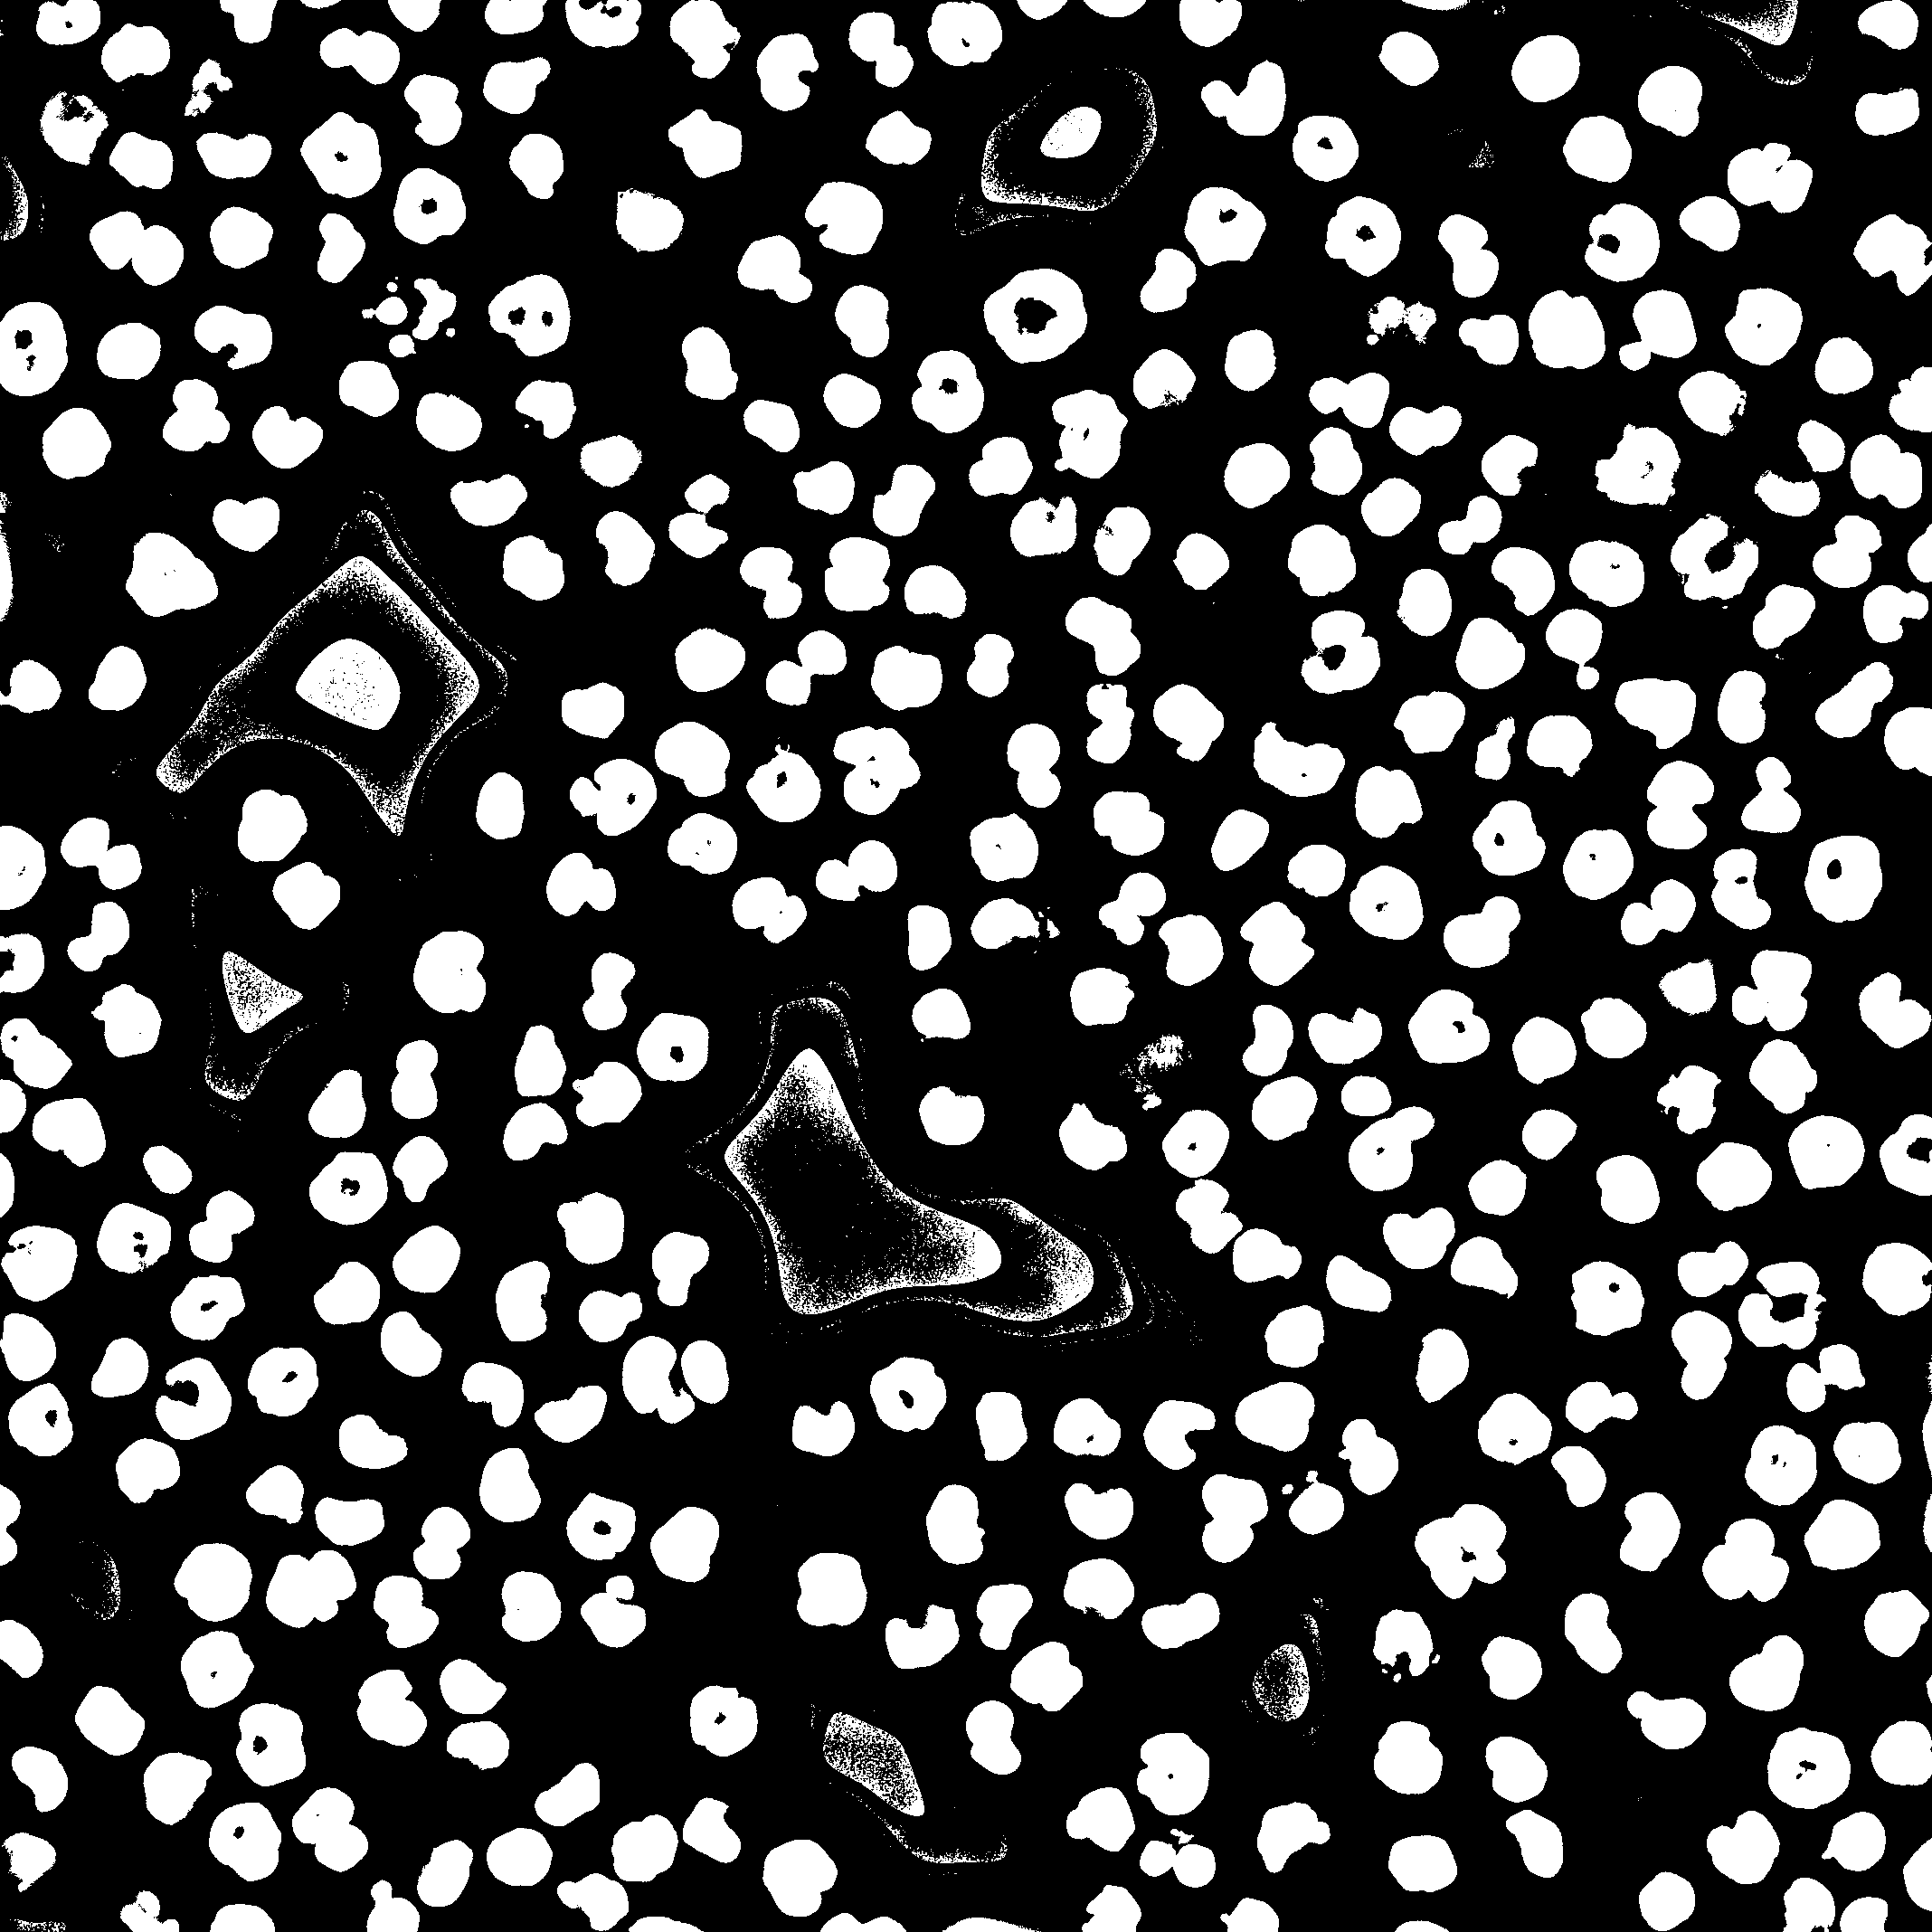
\includegraphics{bilder/segmentation/nuclei-mask/binary_local.png} &
            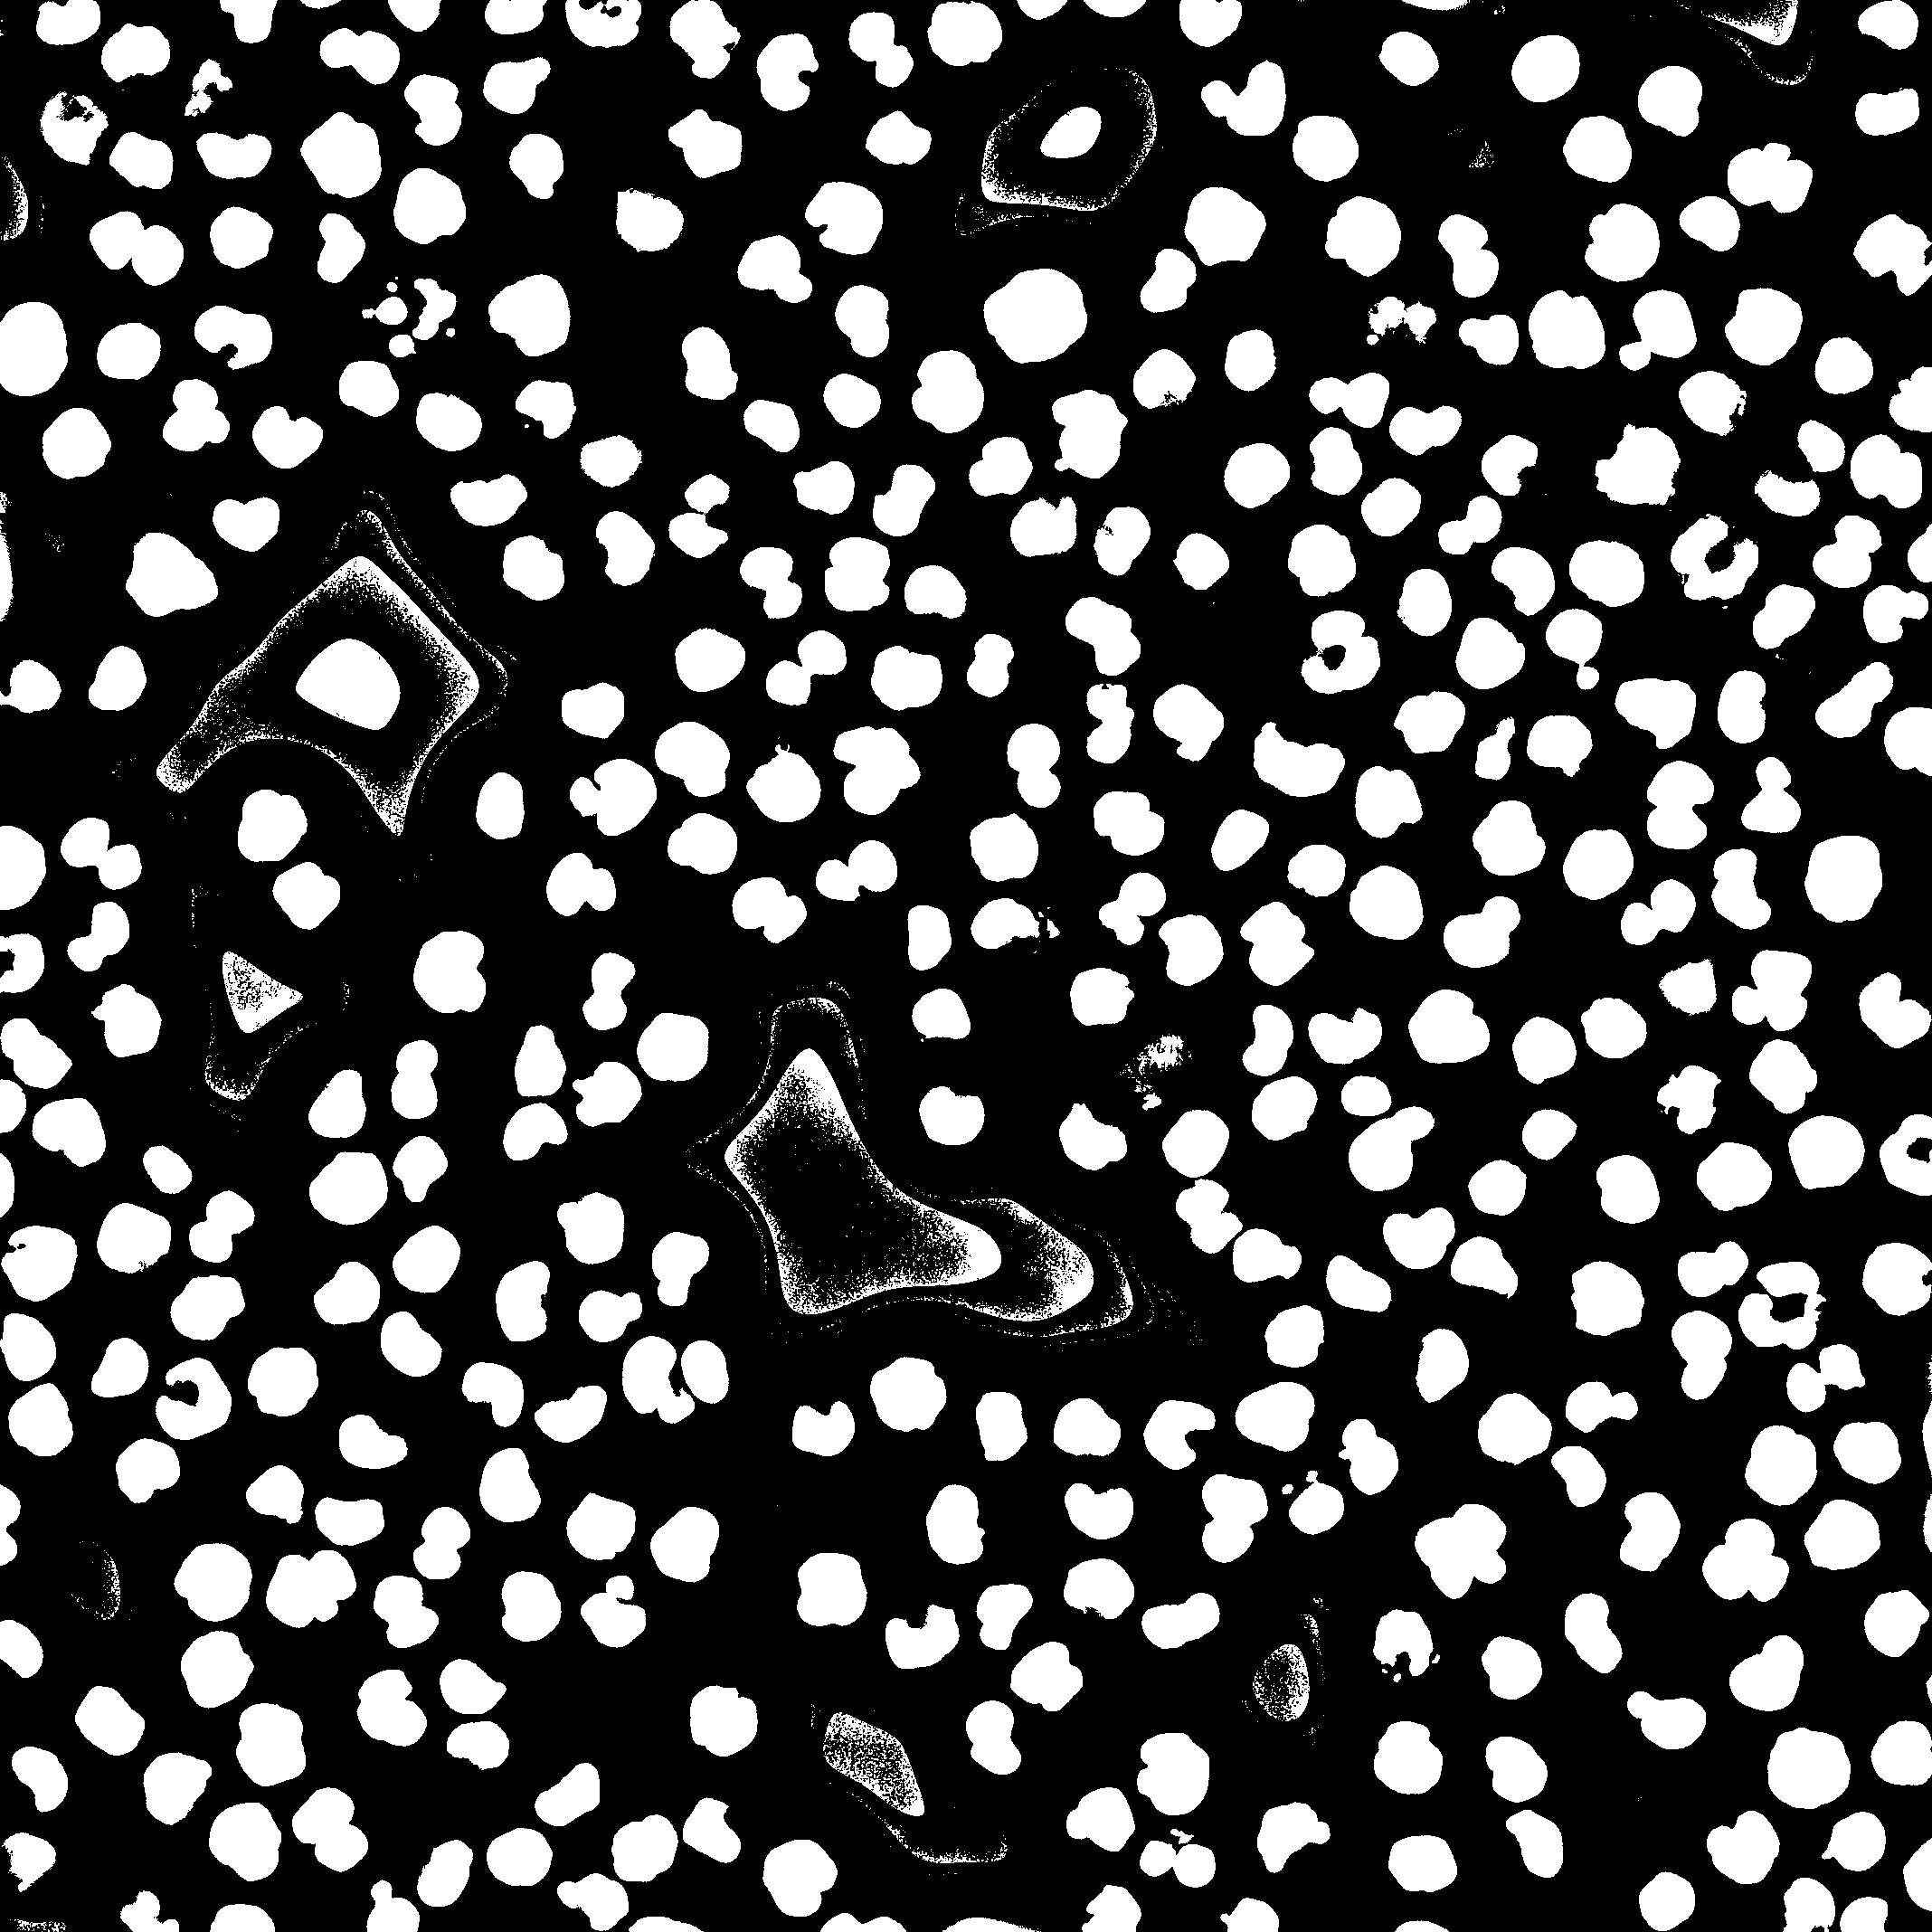
\includegraphics{bilder/segmentation/nuclei-mask/filled_holes.png} & 
            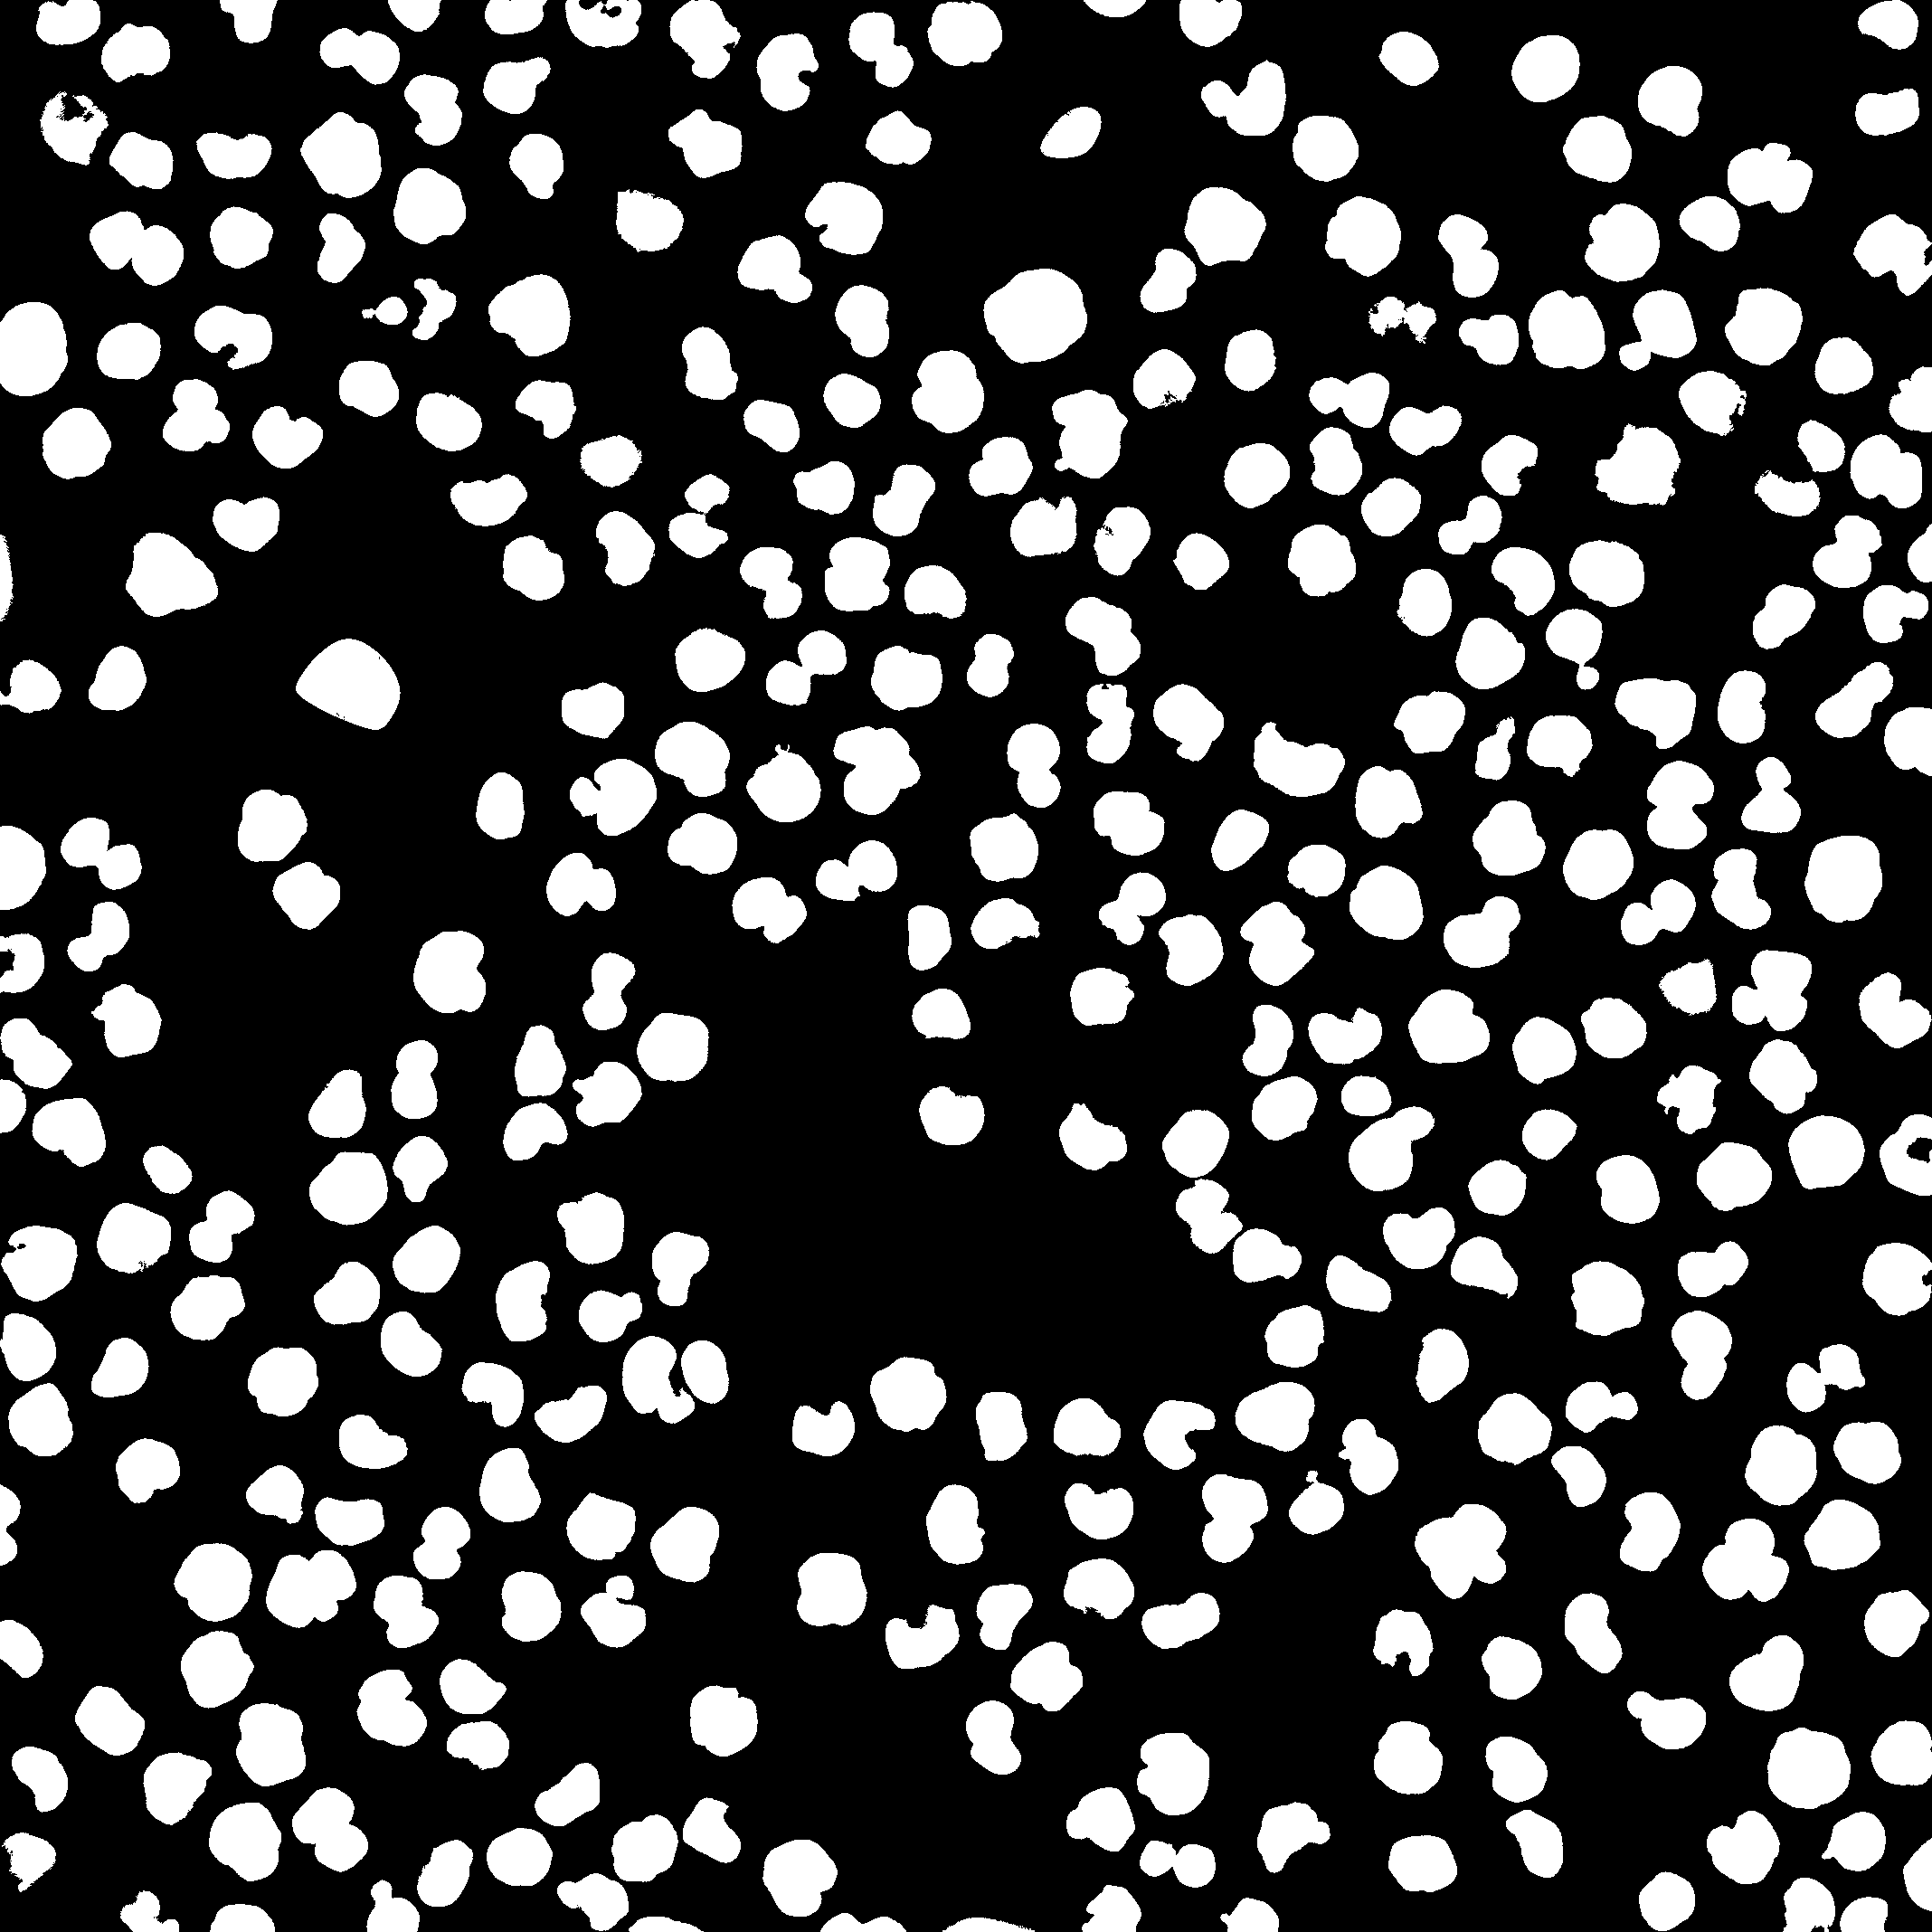
\includegraphics{bilder/segmentation/nuclei-mask/mask.png}
        \end{tabularx}
    \caption{Fluorescence segmentation}
    \label{fig:segmentation-nuclei-steps}
\end{figure}

A more detailed description of the step 2 of the algorithm (thresholding) as well as the general theory behind it is provided in the next subsection.